% !TeX root = ../bbchallenge-paper.tex

\newpage
\subsection{Weighted FAR (WFAR)}\label{sec:WFAR}

% 1RB---_0RC1LC_1RD1RC_1LE1LD_0RA0LE
% 1RB---_0RC1LB_1RD1RC_1LE1LD_0RA0LE
% 1RB---_0RC1RC_1RD1RC_1LE1LD_0RA0LE
% 1RB---_0RC1RC_1RD1RB_1LE1LD_0RA0LE *
% 1RB1RA_1LC1LB_0RD0LC_1RE---_0RA1RA
% 1RB1RA_1LC1LB_0RD0LC_1RE---_0RA1LA
% 1RB1RA_1LC1LB_0RD0LC_1RE---_0RA1LE
% 1RB1RE_1LC1LB_0RD0LC_1RE---_0RA1RA
% 1RB1RA_1LC1LE_0RD0LC_1RE---_0RA1LB
% 1RB---_0RC1LD_1RD1RC_1LE1LB_0RA0LE
% 1RB1RE_1LC1LB_0RD0LC_1LE---_0RA1RA
% 1RB---_0LC1LC_1LD1LB_1RE1RD_0LA0RE
% 1RB1LC_1LC1RA_0LE0LD_0RA1RD_---0LC *
% 1RB1LC_1LB1RA_0LE0LD_0RA1RD_---0LC
% 1RB0RC_1LC0LE_0LD0LB_1RA---_1LB0RD
% 1RB0RE_0RC0RA_1LD---_1LA0LB_1RA0LC
% 1RB0LD_1RC0RA_0RD0RB_1LE---_1LB0LC *
\usetikzlibrary{automata, positioning, arrows.meta}
\begin{figure}[h]
    \centering
    \begin{minipage}[t]{0.22\textwidth}
        \raggedright
        (a) Turing machine \\
        \centering
        \vspace{0.3em}
        \begin{tabular}{ccc}
            \toprule
                    & \textbf{0} & \textbf{1} \\
            \midrule
            \stateA & 1R\stateB  & ---        \\
            \stateB & 0R\stateC  & 1L\stateC  \\
            \stateC & 1R\stateD  & 1R\stateC  \\
            \stateD & 1L\stateE  & 1L\stateD  \\
            \stateE & 0R\stateA  & 0L\stateE  \\
            \bottomrule
        \end{tabular}

        \vspace{2em}
        \raggedright
        (b) Space-time diagram \\
        \centering
        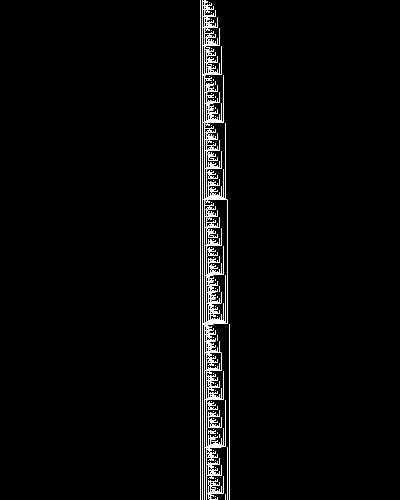
\includegraphics[width=1.2\linewidth]{figures/space-time-diagrams/counter_wfar.png}
    \end{minipage}
    \hfill
    \begin{minipage}[t]{0.30\textwidth}
        \raggedright
        (c) Left weighted automaton \\
        \vspace{0.5em}
        \centering
        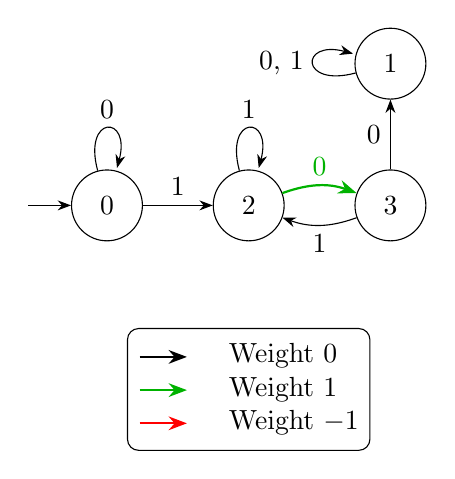
\begin{tikzpicture}[->, >=Stealth, auto, node distance=1.8cm, every node/.style={scale=1}]
            \tikzset{
                state/.style={
                        circle, draw, minimum size=0.9cm, inner sep=1pt
                    }
            }

            % States
            \node[state] (0) {0};
            \node[state] (2) [right of=0] {2};
            \node[state] (3) [right of=2] {3};
            \node[state] (1) [above of=3] {1};

            % Initial arrow
            \draw[->] (-1,0) -- (0);

            % Transitions
            \draw[->, black] (0) edge[loop above] node{0} (0);
            \draw[->, black] (0) edge node{1} (2);

            \draw[->, black] (2) edge[loop above] node{1} (2);
            \draw[->, black, bend left=20] (3) to node{1} (2);
            \draw[->, green!70!black, thick, bend left=20] (2) to node{0} (3);

            \draw[->, black] (3) edge node{0} (1);
            \draw[->, black] (1) edge[loop left] node{0, 1} (1);

            % Compact and aligned legend
            \node[draw, below=1.1cm of 2, inner sep=4pt, rounded corners] (legend) {
                \begin{tabular}{@{}rl@{}}
                    \tikz[baseline=-0.5ex]\draw[->, black, thick] (0,0) -- +(0.6,0);          & \;Weight 0    \\
                    \tikz[baseline=-0.5ex]\draw[->, green!70!black, thick] (0,0) -- +(0.6,0); & \;Weight 1    \\
                    \tikz[baseline=-0.5ex]\draw[->, red, thick] (0,0) -- +(0.6,0);            & \;Weight $-1$
                \end{tabular}
            };
        \end{tikzpicture}

        % \vspace{1em}
        % $\rightarrow$ \quad 1\,0\,|\,0\,|\,0\,1 \\
        % \vspace{0.5em}
        % $+\;4$

        \vspace{2.3em}

        \raggedright
        (d) Right weighted automaton \\
        \vspace{0.3em}
        \centering
        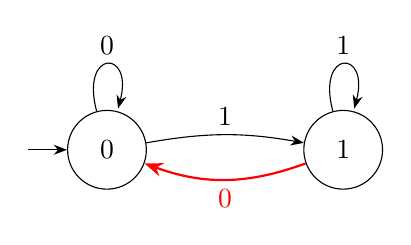
\begin{tikzpicture}[->, >=Stealth, auto, node distance=2cm, every node/.style={scale=1}]
            \tikzset{
                state/.style={
                        circle, draw, minimum size=1cm, inner sep=1pt
                    }
            }

            % % Upper isolated state
            % \node[state] (1top) at (0,2.5) {1};
            % \draw[->] (1top) edge[loop above] node{1} (1top);
            % \draw[->] (1top) edge[loop left] node{0} (1top);

            % Lower automaton
            \node[state] (0) at (0,0) {0};
            \node[state] (2) at (3,0) {1};

            \draw[->] (0) edge[loop above] node{0} (0);
            \draw[->] (2) edge[loop above] node{1} (2);

            \draw[->] (0) edge[bend left=10] node{1} (2);
            \draw[->, red, bend left=20, thick] (2) to node[below]{0} (0);

            % Initial state arrow
            \draw[->] (-1,0) -- (0);
        \end{tikzpicture}



        % \vspace{0.5em}
        % \raggedright
        % (e) Example \\
        % \centering
        % \vspace{-1.5em}
        % \begin{align*}
        %     \texttt{101010} \quad & \text{\stateC}1\quad & \texttt{01}         & \\
        %     \rightarrow \quad     & \text{\stateC}1\quad & \leftarrow          & \\
        %     [3] \quad             & \text{\stateC}1\quad & [0]                 & \\
        %     W_\text{left} = 3     &                      & W_\text{right} = -1   \\
        % \end{align*}

        % \vspace{1em}
        % % $\leftarrow$ \quad D1\,\,0\,1\,0\,1 \\
        % % \vspace{0.5em}
        % % $-\;2$
    \end{minipage}
    \hfill
    \begin{minipage}[t]{0.32\textwidth}
        % \vspace{5em}
        \raggedright
        (e) Accepted weighted configurations \\
        \vspace{-1em}
        \footnotesize
        \begin{minipage}[t]{0.48\textwidth}
            \begin{align*}
                 & [0]\; \text{\stateA}0\; [0];\; W = 0    \\
                 & [3]\; \text{\stateA}0\; [0];\; W \geq 0 \\
                 & [3]\; \text{\stateA}0\; [1];\; W \geq 1 \\
                 & [2]\; \text{\stateB}0\; [0];\; W \geq 0 \\
                 & [2]\; \text{\stateB}0\; [1];\; W \geq 1 \\
                 & [2]\; \text{\stateB}1\; [0];\; W \geq 1 \\
                 & [2]\; \text{\stateB}1\; [1];\; W \geq 1 \\
                 & [2]\; \text{\stateC}0\; [0];\; W \geq 1 \\
                 & [2]\; \text{\stateC}0\; [1];\; W \geq 2 \\
                 & [3]\; \text{\stateC}0\; [0];\; W \geq 1 \\
                 & [3]\; \text{\stateC}0\; [1];\; W \geq 2 \\
                 & [2]\; \text{\stateC}1\; [0];\; W \geq 1 \\
                 & [2]\; \text{\stateC}1\; [1];\; W \geq 1 \\
                 & [3]\; \text{\stateC}1\; [0];\; W \geq 2 \\
                 & [3]\; \text{\stateC}1\; [1];\; W \geq 1 \\
            \end{align*}
        \end{minipage}
        \hfill
        \vrule width 0.5pt
        \hfill
        \begin{minipage}[t]{0.48\textwidth}
            \begin{align*}
                 & \;[2]\; \text{\stateD}0\; [0];\; W \geq 1 \\
                 & \;[2]\; \text{\stateD}0\; [1];\; W \geq 1 \\
                 & \;[2]\; \text{\stateD}1\; [0];\; W \geq 2 \\
                 & \;[2]\; \text{\stateD}1\; [1];\; W \geq 2 \\
                 & \;[3]\; \text{\stateD}1\; [1];\; W \geq 2 \\
                 & \;[0]\; \text{\stateE}0\; [0];\; W = 0    \\
                 & \;[2]\; \text{\stateE}0\; [0]; W \geq -1  \\
                 & \;[0]\; \text{\stateE}1\; [0];\; W = 0    \\
                 & \;[2]\; \text{\stateE}1\; [0];\; W \geq 0 \\
                 & \;[2]\; \text{\stateE}1\; [1];\; W \geq 1 \\
                 & \;[3]\; \text{\stateE}1\; [0];\; W \geq 0 \\
                 & \;[3]\; \text{\stateE}1\; [1];\; W \geq 1 \\
            \end{align*}
        \end{minipage}


    \end{minipage}

    \caption{TODO}
\end{figure}